\documentclass[12pt,A4]{article}
\usepackage{fullpage}
\usepackage[top=2cm, bottom=4.5cm, left=2.5cm, right=2.5cm]{geometry}
\usepackage{amsmath,amsthm,amsfonts,amssymb,amscd}
\usepackage{lastpage}
\usepackage{enumerate}
\usepackage{fancyhdr}
\usepackage{mathrsfs}
\usepackage{xcolor}
\usepackage{graphicx}
\usepackage{listings}
\usepackage{hyperref}
\usepackage{cancel}

%\hypersetup{%
%  colorlinks=true,
%  linkcolor=blue,
%  linkbordercolor={0 0 1}
%}
 
 \lstset{
    basicstyle=\ttfamily,
    columns=fullflexible,
    frame=single,
    breaklines=true,
    prebreak=\mbox{\textcolor{black}{...}\space},
 }
 
\renewcommand\lstlistingname{Algorithm}
\renewcommand\lstlistlistingname{Algorithms}
\def\lstlistingautorefname{Alg.}

%\lstdefinestyle{Python}{
%    language        = Python,
%    frame           = lines, 
%    basicstyle      = \footnotesize,
%    keywordstyle    = \color{blue},
%    stringstyle     = \color{green},
%    commentstyle    = \color{red}\ttfamily
%}

\setlength{\parindent}{0.0in}
\setlength{\parskip}{0.05in}

% Edit these as appropriate
\newcommand\course{EECE 5644}
\newcommand\hwnumber{1}                  % <-- homework number
\newcommand\authName{Nicolas Tedori}           % <-- NetID of person #1
%\newcommand\NetIDb{netid12038}           % <-- NetID of person #2 (Comment this line out for problem sets)
\newcommand{\dueDate}{September 29, 2019}
\newcommand{\classSection}{Prof. David Brady}
\newcommand{\tpose}{^\mathbf{T}}

\pagestyle{fancyplain}
\headheight 35pt
\lhead{\authName \\ \dueDate}
%\lhead{\NetIDa\\\NetIDb}                 % <-- Comment this line out for problem sets (make sure you are person #1)
\chead{\href{https://github.com/niclad/eece5644/tree/master/homework-1}{\textbf{\Large Homework \hwnumber}}}
\rhead{\course \\ \classSection}
\lfoot{}
\cfoot{}
\rfoot{\small Tedori \thepage \hspace{1pt} of \pageref{LastPage}}
\headsep 1.5em

\begin{document}

\textbf{Question 1}

\begin{enumerate}
    \item If \( E[x] = \mu\), show that \( E[(x - \mu)^2] = E[x^2] - \mu^2\).
    
    \begin{align*}
            E[(x - \mu)^2] &= E[X^2 - 2x\mu + \mu ^2] \\
            &= E[x^2] - 2E[x]\mu + \mu^2 \\
            &= E[x^2] 2\mu^2 + \mu^2 = \boxed{E[x^2] - \mu^2}
    \end{align*}
    
    \item If \( E[\mathbf{x}] = \mu\), show that \( E[(\mathbf{x} - \mu)(\mathbf{x} - \mu)^\mathbf{T}] = E[\mathbf{xx}^\mathbf{T}] - \mu\mu^\mathbf{T}\). \label{q1p2}
    
    \begin{align*}
            E[(\mathbf{x} - \mu)(\mathbf{x} - \mu)^\mathbf{T}] &= E[\mathbf{xx^T} - \mathbf{x}\mu^\mathbf{T} - \mu\mathbf{x^T} + \mu\mu^\mathbf{T}] \\
            &= E[\mathbf{xx^T} - E[\mathbf{x}]\mu^\mathbf{T} - \muE[\mathbf{x}]^\mathbf{T} + \mu\mu^\mathbf{T} \\
            &= E[\mathbf{xx^T}] - \mu\mu^\mathbf{T} - \cancel{\mu\mu\tpose} + \cancel{\mu\mu\tpose} \\
            &= \boxed{E[ \mathbf{xx}^ \mathbf{T}] - \mu \mu ^ \mathbf{T}}
    \end{align*}
\end{enumerate}

\textbf{Question 2}

\(p(x|L=l) \propto e^{-|x - a_l| / b_l}\) for \(l \in 1, 2\) and \(b_l > 0\).

\begin{enumerate}
    \item Finding the normalization factor \textit{k}. It is known that \(1 = \int_{-\infty}^{\infty}p(x|L=l) \ \mathrm{d}x\).
    
    \begin{align*}
        1 &= \int_{-\infty}^{\infty} \! ke^{-|x - a_l| / b_l} \\
        \therefore \ 1 &= \frac{-b_lk(x-a_l)e^{-|x-a_l|/b_l}}{|x-a_l|} + C \ \Big|_{-\infty}^{\infty} \\
         &= 2 \cdot \frac{-b_lk(x-a_l)e^{-|x-a_l|/b_l}}{|x-a_l|} + C \ \Big|_{a_l}^{\infty} \\
        \therefore \ 1 &= 2b_lk \cdot \left(\lim_{x \to \infty}\left[ \frac{-(x)e^{-|x|/b_l}}{|x|} \right] +
        \lim_{x \to 0}\left[ \frac{(x)e^{-|x|/b_l}}{|x|}\right]\right) \\
        1 &= 2b_lk \longrightarrow \boxed{k = \frac{1}{2b_l}}
    \end{align*}
    Therefore, via symmetry, the normalization factor is \(1/2b_l\).
    % note for the limits, x either = inf - a_l OR a_l - a_l
    \item Log-likelihood ratio between the two classes for a given \textit{x}, \(l(x) = \ln[p(x|L = 1)] - \ln[p(x|L = 2)]\).
    
    \begin{align*}
        l(x) = \ln\left[\frac{p(x|L=1)}{p(x|L=2)}\right] &= \ln\left[ \frac{\frac{1}{2b_1} \cdot e^{-|x-a_1|/b_1}}{\frac{1}{2b_2} \cdot e^{-|x-a_2|/b_2}} \right] \\
        e^{\ln\left[\frac{p(x|L=1)}{p(x|L=2)}\right]} &= e^{\ln\left[ \frac{\frac{1}{2b_1} \cdot e^{-|x-a_1|/b_1}}{\frac{1}{2b_2} \cdot e^{-|x-a_2|/b_2}} \right]}\\
        \frac{p(x|L=1)}{p(x|L=2)} &= \frac{\frac{1}{2b_1} \cdot e^{-|x-a_1|/b_1}}{\frac{1}{2b_2} \cdot e^{-|x-a_2|/b_2}} \\
        &= \boxed{\frac{b_2}{b_1} \cdot e^{(-|x-a_1|/b_1) + (|x-a_2|/b_2)}}
    \end{align*}
    
    \item A plot, where \(a_1 = 0, b_1 = 1\) and \(a_2 = 1, b_2 = 2\). Code available \href{https://github.com/niclad/eece5644/blob/master/homework-1/q2p3.m}{\textit{\underline{here}}}.
        $$l(x) = 2 \cdot e^{(-2\cdot|x|+|x-1|)/2}$$
        \begin{figure}[h]
            \centering
            \includegraphics[scale=0.75]{q2p3.eps}
            \label{fig:my_label}
        \end{figure}
        \begin{center}
            Code for question 2 problem 3 avialable at: \url{https://github.com/niclad/eece5644/blob/master/homework-1/q2p3.m}
        \end{center}
\end{enumerate}{}

%Question 3
\textbf{Question 3}

It is given that: Prior probabilities are \(P(L=1) = P(L=2) = 1/2\) and that \textit{x} is in \(Uniform[a, b]\) for class 1 and \(Uniform[r, t]\) for class 2. \\\\
\(a < r < b < t\) therefore the pdfs of $p(x|L=1)$ and $p(x|L=2)$ overlap.\\\\
Minimum probability of error classification rule: \\

Given uniform densities, it is known that:
$$p(x|L=1)=\frac{1}{b-a}$$
$$p(x|L=2)=\frac{1}{t-r}$$
\begin{equation} \label{eq:1}
    \therefore \ p(L=1|x)=\frac{p(x|L=1)\cdot p(L=1)}{p(x)}=\frac{1}{2(b-a)p(x)} \quad \textrm{If \textit{x} is in the range $[a, b]$.}
\end{equation}
\begin{equation} \label{eq:2}
    p(L=2|x)=\frac{p(x|L=2)\cdot p(L=2)}{p(x)}=\frac{1}{2(t-r)p(x)} \quad \textrm{If \textit{x} is in the range $[r, t]$.}
\end{equation}

$$\textrm{If \textit{x} is not in the range $[a, t]$, then } p(x|L=1) = p(x|L=2) = 0 \textrm{ and } p(error|x) = 0$$
$$\textrm{If \textit{x} is in the range $[a, r)$, then } p(x|L=2) = 0 \textrm{ and } p(error|x) = 0$$
$$\textrm{If \textit{x} is in the range $(b, t]$, then } p(x|L=1) = 0 \textrm{ and } p(error|x) = 0$$

If \textit{x} is in the range [r, b], then:
$$p(error) = \int_{-\infty}^{\infty} p(error|x) \cdot p(x)\ \mathrm{d}x$$

If $b-a > t-r$, then $p(L=1|x) < p(L=2|x)$ (by equation \ref{eq:1}):
\begin{align*}
    p(error) &= \int_{r}^{b} p(L=1|x) \cdot p(x)\ \mathrm{d}x \\
    &= \int_{r}^{b} \frac{1}{2(b-a)\cancel{p(x)}} \cdot \cancel{p(x)}\ \mathrm{d}x \\
    &= \frac{x}{2(b-a)} + C \ \Big|_r^b = \frac{b-r}{2(b-a)}
\end{align*}

If $b-a < t-r$, then $p(L=1|x) > p(L=2|x)$ (by equation \ref{eq:2}):
\begin{align*}
    p(error) &= \int_{r}^{b} p(L=2|x) \cdot p(x)\ \mathrm{d}x \\
    &= \int_{r}^{b} \frac{1}{2(t-r)\cancel{p(x)}} \cdot \cancel{p(x)}\ \mathrm{d}x \\
    &= \frac{x}{2(t-r)} + C \ \Big|_r^b = \frac{t-r}{2(b-a)}
\end{align*}

\begin{equation*}
    \therefore \ \boxed{p(error) = \begin{cases}
    \frac{b-r}{2(b-a)}, & \text{if $r\leq x\leq b$ and $b-a \geq t-r$} \\
    \frac{b-r}{2(t-r)}, & \text{if $r\leq x\leq b$ and $b-a < t-r$} \\
    0,                  & \text{O.W.}
    \end{cases}}
\end{equation*}

\textbf{Question 4} \\
Two classes with equal class prior probabilities. Gaussian class-conditioned pdfs $N(0, 1)$ and $N(\mu, \sigma^2)$.

\begin{enumerate}
    \item Classification/decision rule. Minimum probability of error will occur at $P(x|L=1) = P(x|L=2)$, Bayes optimal decision boundary. It is given that $\mu_1=0, \sigma_1^2=1$ and $\mu_2=\mu, \sigma_2^2=\sigma^2$. By Gaussian R.V.:
    \begin{equation*}
    P(x|L=1) = \frac{1}{\sqrt{2\pi}} \cdot e^{-\frac{1}{2} \cdot x^2} = \frac{1}{\sigma\sqrt{2\pi}} \cdot e^{-\frac{1}{2} \cdot \frac{(x-\mu)^2}{\sigma^2}} = P(x|L=2)
    \end{equation*}
    \begin{align*}
        \cancel{\frac{1}{\sqrt{2\pi}}} \cdot e^{-\frac{1}{2} \cdot x^2} &= \cancel{\frac{1}{\sqrt{2\pi}}} \cdot \frac{1}{\sigma} \cdot e^{-\frac{1}{2} \cdot \frac{(x-\mu)^2}{\sigma^2}}\\
        \ln(\sigma) - \frac{1}{2}x^2 &= -\frac{(x-\mu)^2}{2\sigma^2} \\
        0 &= -(x-\mu)^2 + \sigma^2x^2 - 2\sigma^2\ln(\sigma)\\
        0 &= \sigma^2x^2 - x^2 + 2\mu x - \mu^2 - 2\sigma^2\ln(\sigma) \\
        0 &= (\sigma^2 - 1)x^2 + 2\mu x - \mu^2 - 2\sigma^2\ln(\sigma)
    \end{align*}
    Solving for \textit{x}:
    $$\boxed{x = \frac{-\mu \pm \sigma\sqrt{\mu^2 + 2\ln(\sigma)(\sigma^2 - 1)}}{\sigma^2 - 1}}$$
    
    \item For $\mu_2 = 1, \sigma_2^2 = 2$ plot $p(x|L=l)$ for $l\in 1, 2$ and $p(L=l|x)$ for $l\in 1, 2$
    $$P(x|L=1) = \frac{1}{\sqrt{2\pi}} \cdot e^{-\frac{1}{2} \cdot x^2}$$
    $$P(x|L=2) = \frac{1}{\sigma\sqrt{2\pi}} \cdot e^{-\frac{1}{2} \cdot \frac{(x-\mu)^2}{\sigma^2}}$$
    $$P(L=l|x)=\frac{P(x|L=l) \cdot P(L=l)}{P(x)}$$
    Given that $P(L=1) = P(L=2)$ and that $P(x) = P(x|L=1)P(L=1) + P(x|L=2)P(L=2)$, then $P(x) = P(L=1)[P(x|L=1) + P(x|L=2)]$
    
    $$\therefore \ P(L=l|x)=\frac{P(x|L=l) \cdot \cancel{P(L=l)}}{\cancel{P(L=l)}[P(x|L=1) + P(x|L=2)]}$$
    $$\therefore \ P(L=1|x)=\frac{P(x|L=1)}{P(x|L=1) + P(x|L=2)}$$
    $$P(L=2|x)=\frac{P(x|L=2)}{P(x|L=1) + P(x|L=2)}$$
    
    \begin{figure}[h]
    \centering
    \begin{minipage}{0.5\textwidth}
        \centering
        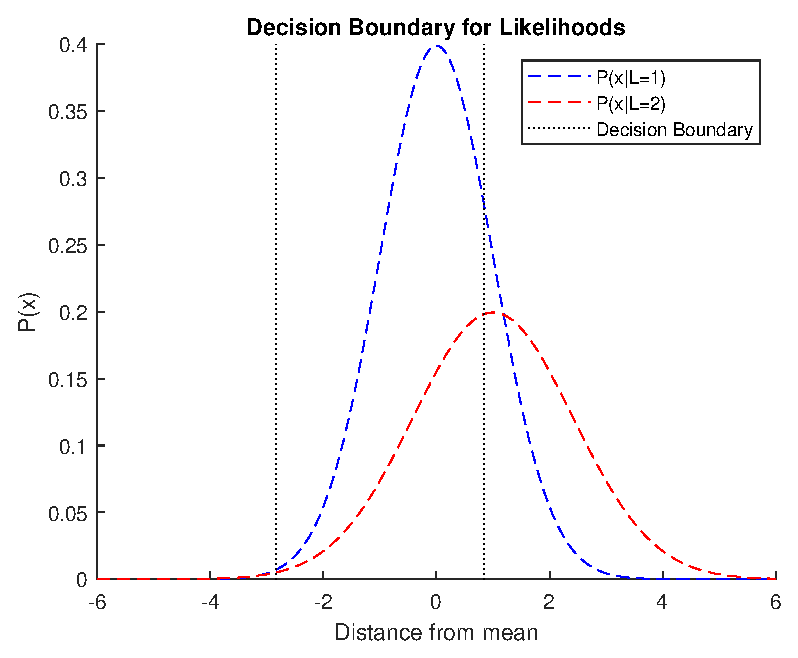
\includegraphics[width=0.9\textwidth]{plot1.eps} % first figure itself
    \end{minipage}\hfill
    \begin{minipage}{0.5\textwidth}
        \centering
        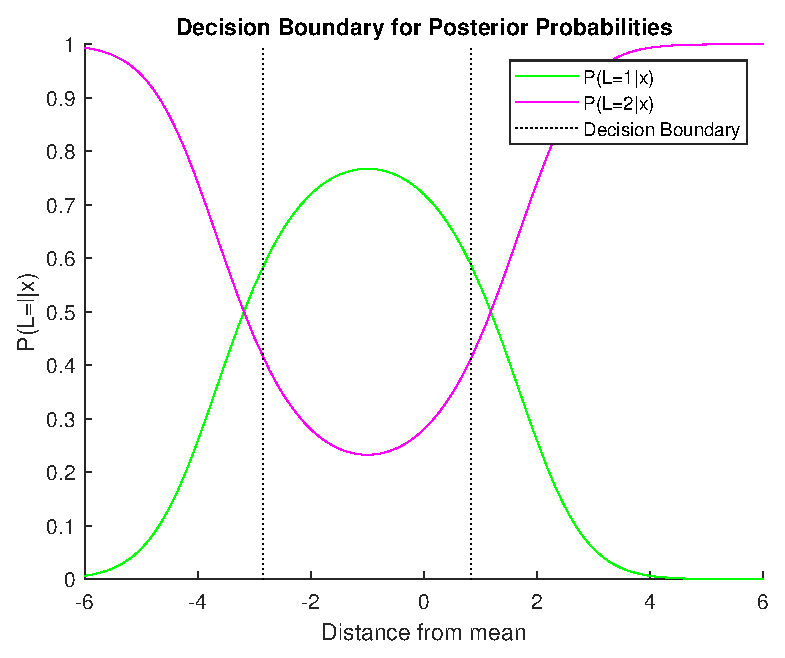
\includegraphics[width=0.9\textwidth]{plot2.eps} % second figure itself
    \end{minipage}
\end{figure}

\begin{center}
    Code for question 4, problem 2 available at: \url{https://github.com/niclad/eece5644/blob/master/homework-1/q4p2.m}
\end{center}

    \item Estimation of the minimum $p(error)$:
    
    Given that $P(x|L=1)=P(x|L=2)=0.84$ and $P(L=1|x) = P(L=2|x)=0.84$ for $x=-1+\sqrt{2+2\ln(2)}$\\
    \begin{align*}
        P(error) &= \int_{-\infty}^{\infty}\min[P(L=1|x), P(L=2|x)]\cdot p(x)\ \mathrm{d}x \\
        &= \int_{-\infty}^{0.84}P(L=2|x)\cdot P(x) \ \mathrm{d}x + \int_{0.84}^{\infty}P(L=1|x)\cdot P(x) \ \mathrm{d}x
    \end{align*}
    
    Given that $P(L=l|x)\cdot P(x) = P(x|L=l)\cdot P(L=l)$ by \href{https://en.wikipedia.org/wiki/Bayes\%27_theorem}{Bayes' Theorem}:
    
    $$P(error) = \int_{-\infty}^{0.84}P(x|L=2)\cdot P(L=2) \ \mathrm{d}x + \int_{0.84}^{\infty}P(x|L=1)\cdot P(L=2) \ \mathrm{d}x$$
    
    Given that $P(L=1)=P(L=2)$:
    \begin{align*}
        P(error) &= \int_{-\infty}^{0.84}P(x|L=2)\cdot P(L=2) \ \mathrm{d}x + \int_{0.84}^{\infty}P(x|L=1)\cdot P(L=2) \ \mathrm{d}x \\
        &= P(L=1)\cdot \left[ \int_{-\infty}^{0.84}P(x|L=2) \ \mathrm{d}x + \int_{0.84}^{\infty}P(x|L=1) \ \mathrm{d}x \right] \\
        &= 0.5 \cdot \left[ \int_{-\infty}^{0.84}\frac{1}{\sqrt{4\pi}} \cdot e^{-\frac{1}{2} \cdot \frac{(x-1)^2}{2}} \ \mathrm{d}x + \int_{0.84}^{\infty}\frac{1}{\sqrt{2\pi}} \cdot e^{-\frac{1}{2} \cdot x^2} \ \mathrm{d}x \right] \\
        &\quad \vdots \\
        &\approx 0.5 \cdot \left[ 0.455 + 0.201\right] \\
        P(error) &\approx 0.328
    \end{align*}
    
    This procedure starts by finding the optimal Bayes Decision Boundary where the two curves intersect. Using the property that the probability of error is proportional to the minimum area under the Gaussian distribution. Given that the two curves intersect, the error calculation takes the integral of the minimum from $-\infty$ up until the boundary and then adds the integral of the new minimum until $\infty$.
    
    \item What if $\mu_2 = 0$ and $\sigma_2^2\gg 1$? \\
    Given that the variance ($\sigma^2$) is a measure of the closeness of the data to the mean, if the variance grew to much larger than one, then Normal Distribution would become less ``peaky,'' spreading out over the \textit{x}-axis. As the variance becomes larger, the decision boundary shifts towards the right. However, with a mean of 0, the error calculation with have to take in additional bounds as there will be more than one place where the minimum switches between classes. A situation like this might arise when comparing commute distances in a city. People may either live down the street from their office in an apartment or live in a suburb 45 minutes away. Accounting for an entire city might yield data that follows a similar shape with a large variance.
\end{enumerate}

\textbf{Question 5}

\newcommand{\mbold}[1]{\boldsymbol{\mathrm{#1}}}
Pdf of an \textit{n}-dimensional random vector drawn from $N(\boldsymbol{\mu}, \boldsymbol{\Sigma})$ is
$$p(\boldsymbol{\zeta}) = (2\pi)^{-n/2}|\boldsymbol{\Sigma}|^{-1/2}e^{-(1/2)(\boldsymbol{\zeta}-\boldsymbol{\mu})^T\boldsymbol{\Sigma}^{-1}(\boldsymbol{\zeta} - \boldsymbol{\mu})}$$

\begin{enumerate}
    \item Determine the pdf of x:
    $$\boldsymbol{\mathrm{x}} = \boldsymbol{\mathrm{Az}} + \boldsymbol{\mathrm{b}}$$
    $$\therefore \ E[\boldsymbol{\mathrm{x}}]=\boldsymbol{\mathrm{b}}$$
    Given that \textbf{z} $\sim N(\boldsymbol{0}, \boldsymbol{\mathrm{I}})$:
    $$E[\boldsymbol{\mathrm{Az}}]=\boldsymbol{\mathrm{A}}E[\boldsymbol{\mathrm{z}}]=0$$
    From \textbf{question 1, problem 2}:
    $$E[\mbold{xx^T}]=E[(\mbold{Az}+\mbold{b})(\mbold{Az}+\mbold{b})^{\mbold{T}}]=\mbold{A}E[\mbold{zz^T}]\mbold{A^T}+\mbold{bb^T}$$
    $$E[\mbold{zz^T}]=\mbold{I}$$
    Variance-covariance of \textbf{x} is:
    $$E[\mbold{xx^T}]-E[\mbold{x}]E[\mbold{x^T}]=E[\mbold{xx^T}]-\mbold{bb^T}=\mbold{AA^T}$$
    $$\boxed{\therefore \ \mbold{x} \sim N(\mbold{b}, \mbold{AA^T})}$$
    
    \item Want to determine a random vector drawn from $N(\mbold{\mu}, \mbold{\Sigma})$ using linear transformation techniques. Find \textbf{A} and \textbf{b} in terms of $\mbold{\mu}$ and $\mbold{\Sigma}$.
    \begin{align*}
        \mbold{A}&=\mbold{\Sigma}^{1/2}\\
        \mbold{b}&=\mbold{\mu}
    \end{align*}
    
    \item Code that produces $N$ samples of iid n-dimensional random vectors $\{x_1,...,x_N\}$ drawn from $N(\mbold{\mu}, \mbold{\Sigma})$.
    \begin{center}
        Code for question 5, problem 3 available at: \url{https://github.com/niclad/eece5644/blob/master/homework-1/q5p3.m}
    \end{center}
    \end{enumerate}
    \newpage
    
\textbf{Code}
All code may be found at \url{https://github.com/niclad/eece5644}, specifically in the \href{https://github.com/niclad/eece5644/tree/master/homework-1}{\ttfamily{homework-1}} directory.
\begin{enumerate}
    \item Question 2, problem 3 code:
    \lstinputlisting[language=Matlab]{q2p3.m}
    \item Question 4, problem 2 code:
    \lstinputlisting[language=Matlab]{q4p2.m}
    \item Question 5, problem 3 code:
    \lstinputlisting[language=Matlab]{q5p3.m}
\end{enumerate}

\end{document}
